\documentclass[10pt]{article}

\usepackage{geometry}
\geometry{margin = 3em,top =6em, headheight=\paperheight}
\usepackage[export]{adjustbox}
\usepackage{array}
\usepackage{amsmath}
\usepackage{amsfonts}
\usepackage{fancyhdr}
\pagestyle{fancy}
\fancyhf{}
\lhead{Algebra II}
\chead{Function Vocabulary}
\rhead{In-class Practices, Page \thepage}
\usepackage{lastpage}
\usepackage{xcolor}
\usepackage{enumitem}
\usepackage{pifont}
\usepackage{graphicx}
\graphicspath{{../img}}
\usepackage{pgfplots}
\pgfplotsset{compat=1.18}

\newcommand{\R}{\mathbb R}
\newcommand{\e}{{\rm e}}
\newcommand{\pobr}[1]{\left\langle#1\right\rangle}
\newcommand{\norm}[1]{\lVert #1 \rVert}
\newcommand{\abs}[1]{\lvert #1 \rvert}

\DeclareMathOperator{\xd}{d\!}
\DeclareMathOperator{\proj}{proj}

\title{}
\date{}

\begin{document}
{\noindent\bf Do Now.}

{\it
Terminology Review:
\begin{itemize}[leftmargin=4em]
\item
Zeros/X-Intercepts: Where the graph crosses the x-axis. 
\item
Y-Intercepts: Where the graph crosses the y-intercepts.
\end{itemize}
}
Let \(f(x) = 2x -3\). Find the zeros and the $y$-intercept of the graph of $f(x)$, then plot the graph.
\vspace{\stretch{1}}

{\noindent\bf Discussion.}

It’s the bottom of the 9th inning with two outs, and the home team is trailing by one run. The crowd at \textit{Victory Field} holds its breath as \textbf{Maya}, the team’s power hitter, steps up to the plate.

The pitcher throws. Maya swings --- \textbf{crack!} She hits the ball high into the air. The ball follows a curved path through the sky, and the team’s motion tracker records its flight path with the following equation:
\[
y = -x^2 +3x +10
\]
where:
\begin{itemize}
    \item \( x \) represents the horizontal distance from home plate,
    \item \( y \) represents the height of the ball above the ground.
\end{itemize}

\begin{enumerate}
    \item When did the ball hit the ground? Find the \textbf{horizontal distances} where the ball was at ground level.
    \vspace{\stretch{1}}
    \item How high was the ball when it left the bat at home plate?
    \vspace{\stretch{1}}
    \clearpage
    \item What was the highest point the ball reached, and how far from home plate did it occur?
    \vspace{\stretch{1}}
    \item Sketch the graph of the ball’s flight. Label the zeros, $y$-intercept, and vertex.
    \vspace{\stretch{1}}
\end{enumerate}


{\noindent \bf Exit Ticket.}

Describe the following graph.

\begin{center}
\begin{tabular}{p{0.5\textwidth}p{0.5\textwidth}}
\parbox{0.5\textwidth}{
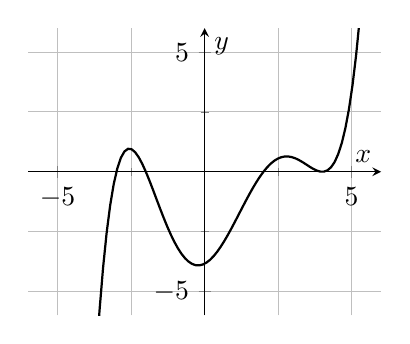
\begin{tikzpicture}
\begin{axis}[
    xlabel={$x$},
    ylabel={$y$},
    grid=both,
    minor tick num=1,
    axis lines=middle,
    domain=-6:6,
    ymin=-6, ymax=6,
    xmin=-6,xmax=6,
    samples=100,
    width=.5\textwidth,
]
\addplot[thick] {(x+3)*(x+2)*(x-2)*(x-4)^2/50};
\end{axis}
\end{tikzpicture}
}&\parbox[c]{0.5\textwidth}{{\bf \large Description}\\[1.5em]
\rule{0.4\textwidth}{0.5pt}\\[1.5em]
\rule{0.4\textwidth}{0.5pt}\\[1.5em]
\rule{0.4\textwidth}{0.5pt}\\[1.5em]
\rule{0.4\textwidth}{0.5pt}\\[1.5em]
\rule{0.4\textwidth}{0.5pt}\\[1.5em]
\rule{0.4\textwidth}{0.5pt}\\[1.5em]
\rule{0.4\textwidth}{0.5pt}\\[1.5em]
}
\end{tabular}
\end{center}

\end{document}